%% This file shows how to use the beamer template ruhuisstijl. It 
%% mimics the corporate and departemental style for the Radboud 
%% University powerpoint presentations. This file contains the 
%% single-file version of the template. 
%% 
%% For comments, questions, and suggestions contact me at 
%% l.onrust@let.ru.nl or visit the github repository on
%% https://github.com/naiaden/presentations/tree/master/ruhuisstijl
%% (this single-file version can be found in the distributed dir)
%%
%% You can distribute and edit the files as you wish, but I'd
%% love to hear of any changes. Also, if you let me know that
%% you are using the template, I can keep you up-to-date on
%% future changes.
%%
%% 10 October 2014: CLS template added
%% 20 October 2014: HLCS template added
%% 28 October 2014: Kaski, PTRS, IMR, SteR templates added
%% 11 November 2014: Group logo added for Language Machines (lama)
%% 25 November 2014: DS, iCIS, IS, MBSD templates 
%% 20 February 2015: Many unoffical options added (thanks Bart Jacobs)
%% 07 March 2016: iCIS Data Science and Software Science added, and small fixes

\documentclass[department=icis, slidenumbers=slide, official=true]{beamerruhuisstijl}
%% The class takes the following optional arguments:
%% notes: {show notes}, {hide notes}, {show only notes} (default = hide notes)
%% official: true, false (default = false)
%% department: datascience, clst, cls, hlcs, kaski, ptrs, imr, ster, ds, is, mbsd, icis (default = RU)
%% grouplogo: lama (default = no group logo)
%% handout
%% slidesperpage: 1, 2, 3, 4, 6 (default = 1)
%%
%% Furthermore, there are some options that do not follow the design
%% or its philosophy. Anyway:
%% slidenumbers: none, slide, relative (default = none)
%% tablecolours: false, true (default = true)
%% alwaysshowauthor: false, true (default = false)
%% alwaysshowdate: false, true (default = false)
%% tocatsectionstart: false, true (default = false)
%% tocatsectionstarttitle: [any string] (default = Overview)
%% showinstitute: false, true (default = false)
%% showdate: false, true (default = false)

\title{Parsing SPL in Haskell}
\subtitle{Aaron van Geffen and Thom Wiggers}
\date{\today}
\author{Aaron van Geffen \and Thom Wiggers}

\usepackage{hyperref}
\usepackage{graphicx}
\usepackage{microtype}
\usepackage{cleveref}

\begin{document}

\begin{frame}
    \titlepage{}
\end{frame}

\begin{frame}{Parsing with Haskell}
    \begin{itemize}
        \item Algebraic Data Structures
        \item Pattern Matching
        \item Parser Combinators
        \item Printer Combinators
        \item Toolchain
            \begin{itemize}
                \item Test-Driven Development
            \end{itemize}
    \end{itemize}
\end{frame}

\begin{frame}{Parser Combinators}
    \begin{itemize}[<+->]
        \item Parsec is the traditional go-to choice
            \begin{itemize}
                \item \ldots but no longer maintained
                \item Many forks are available, with added features
            \end{itemize}
        \item We opted for Megaparsec
            \begin{itemize}
                \item Better testing support
                \item Improved error messages
                \item Unicode support
            \end{itemize}
    \end{itemize}
\end{frame}

\begin{frame}{Parse Tree}
    Haskell's algebraic data types allow for an elegant representation of the 
    parsed programme:
    \pause
    \begin{figure}[b]
        \centering
        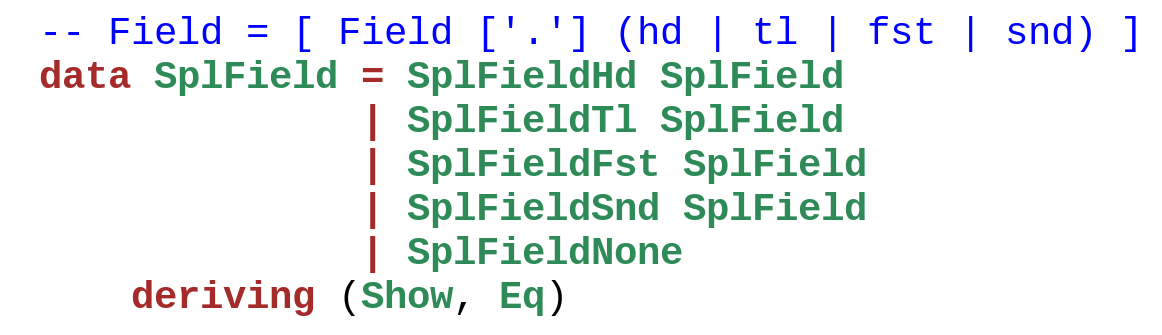
\includegraphics[width=0.9\textwidth]{imgs/splfieldast.png}
    \end{figure}

    This is also an example of where we eliminated left recursion.
\end{frame}

\begin{frame}{Test-Driven Development}
    We can now use the parse tree ADTs to describe the desired behaviour:
    \begin{figure}[b]
        \centering
        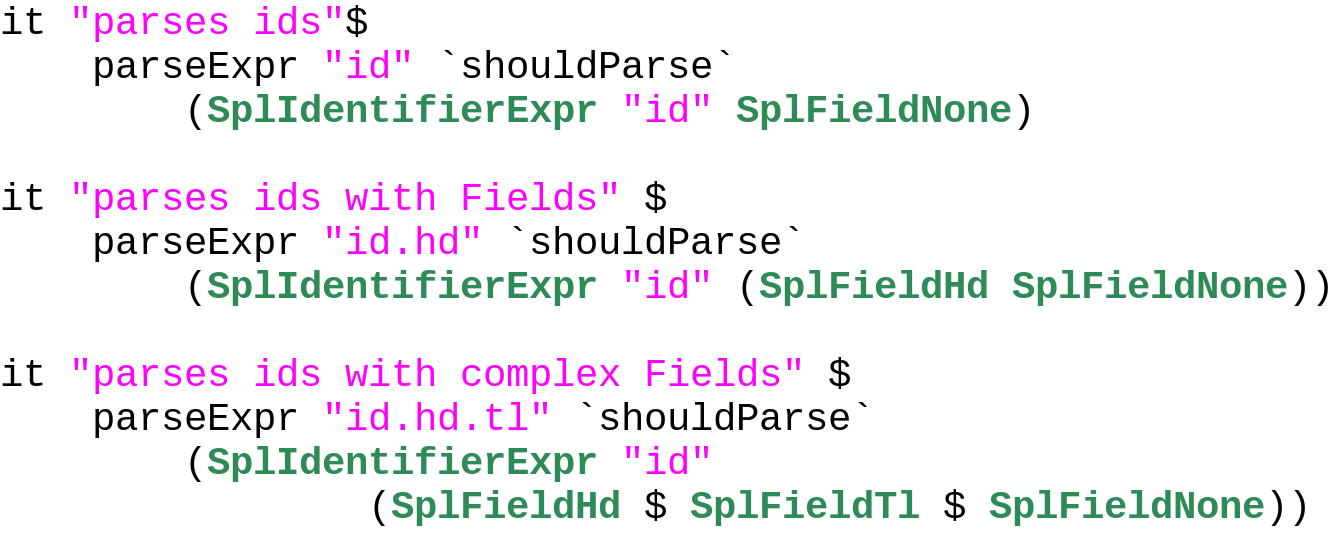
\includegraphics[width=0.9\textwidth]{imgs/fieldspec.png}
    \end{figure}
\end{frame}

\begin{frame}{Implementing the Field Parser}
    \begin{figure}[b]
        \centering
        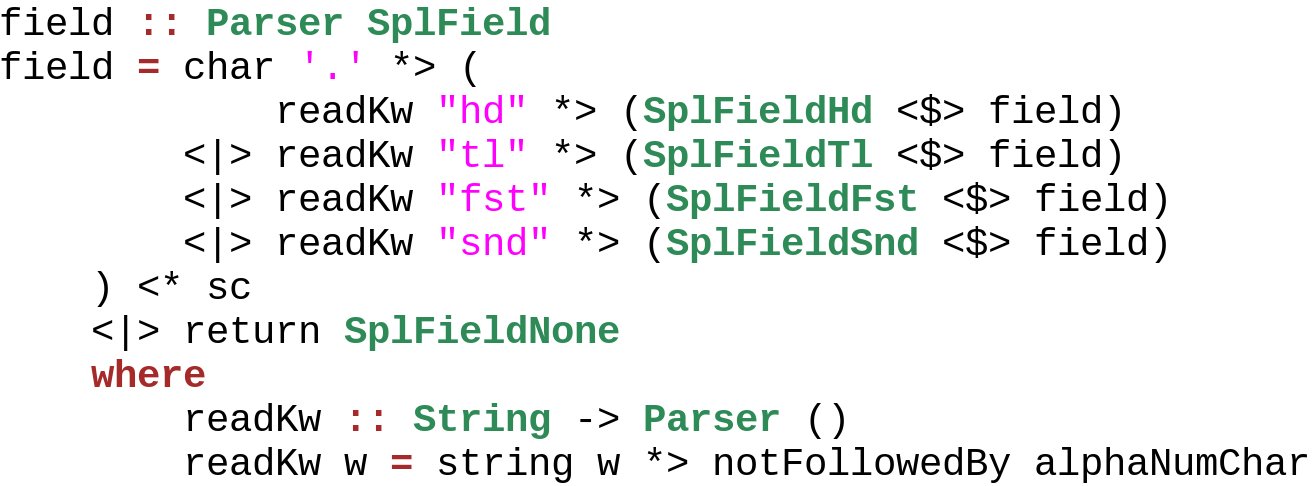
\includegraphics[width=0.9\textwidth]{imgs/fieldimpl.png}
    \end{figure}
\end{frame}

\begin{frame}{Pretty-printing}
    Haskell provides \texttt{Text.PrettyPrint}, a library that allows
    combining text elements, whilst providing tools for indentation and
    other formatting:
    \only<2>{
    \begin{figure}[b]
        \centering
        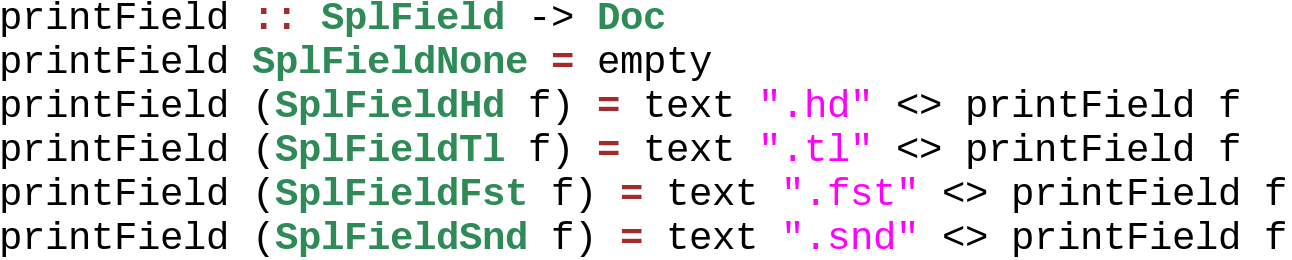
\includegraphics[width=0.9\textwidth]{imgs/printfield.png}
    \end{figure}
    }
    \only<3->{
    \begin{figure}[b]
        \centering
        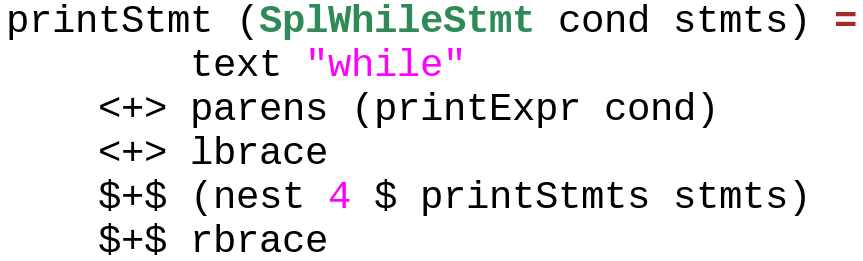
\includegraphics[width=0.60\textwidth]{imgs/printwhile.png}
    \end{figure}
    }

    \only<3->{
    Our test suite also verifies that pretty-printed programs remain parseable.
    }

\end{frame}

\begin{frame}{Going out in style}
    \begin{figure}[b]
        \centering
        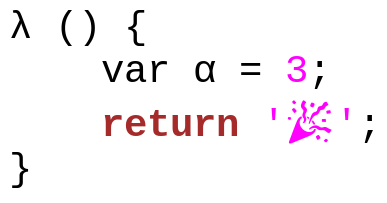
\includegraphics[width=0.9\textwidth]{imgs/lambda.png}
    \end{figure}
\end{frame}

\end{document}
